\chapter{Introduction}
\label{Introduction}
\graphicspath{{Figures/Introduction/}{Figures/Common/}}

It is hard to underestimate the effect that the laser has had since its invention in 1960 \citep{Maiman:1960}.  Although initially motivated by pure scientific curiosity, its unique properties have given it application in an astonishing array of technologies, in addition to its use as a powerful tool in fundamental research.  It is the narrow spectral linewidth, the high spectral intensity, and its large coherence length that give the optical laser such a wide range of applications.  These properties themselves derive from the macroscopic occupation of photons in a single optical mode inside the laser cavity.  With the achievement of Bose-Einstein Condensate (BEC) in 1995 \citep{Anderson:1995vn,Bradley:1995ys,Davis:1995} --- a macroscopic occupation of \emph{atoms} in a single spatial mode --- there has arisen the experimental challenge of producing an atomic analogue of the optical laser: the \emph{atom} laser.  As atoms interact more readily with their environment than photons, atom interferometry has a broad range of applications: to the measurement of electric and magnetic fields in tests of atom and neutron charge neutrality \citep{Arvanitaki:2007}, an application which would be essentially impossible with optical lasers due to the weak photon--photon interaction; to fundamental tests of predictions of General Relativity \citep{Dimopoulos:2007uq}; to the development of gyroscopes \citep{Gustavson:1997}, gradiometers \citep{Snadden:1998,McGuirk:2002} and gravimeters \citep{Peters:2001}, which, while possible using optical lasers, their atomic counterparts are far more compact due to the significantly stronger gravitational interaction.

more broadly and to the development of more compact sensors.  




Although the low kinetic energy of atom lasers would prevent their use 


The differences between an atom laser and an optical laser derive from the inherent differences between photons and atoms: atoms interact much more readily with their environment.  This is both a blessing and a curse.  It is a blessing

 over an optical laser derives from the 



First cw optical laser \citep{Javan:1961}.


The achievement of Bose-Einstein Condensate (BEC) in 1995 \citep{Anderson:1995vn,Bradley:1995ys,Davis:1995} has led to the possibility of creating an analogous source for atoms, which could take advantage of the inherent differences between photons and atoms.  Atoms interact much more readily with their environment, giving atom interferometry applications in fundamental tests of predictions of General Relativity \citep{Dimopoulos:2007uq}, tests of atom and neutron charge neutrality \citep{Arvanitaki:2007}, gyroscopes \citep{Gustavson:1997}, gradiometers \citep{Snadden:1998,McGuirk:2002} and gravimeters \citep{Peters:2001}.  FIXME: How many of these actually use atom lasers, and how many use thermal beams?

The increased interactivity of atoms over photons is both a blessing and a curse: while it is the source of crap.

far more sensitive to fluctuations in external electric or magnetic fields, etc


We need to talk about thermal beams, briefly.



Here goes the motivation.

Steal everything that we can from papers.

\section{Lasers and Atom lasers}

The basic features necessary for a continuous atom laser are analogous to the features of a continuous optical laser: a resonator, a lasing mode, an outcoupling process, and a Bose-stimulated pumping mechanism (see \figureref{Introduction:LaserAtomLaserComparison}).  The first three of these features are well understood for an atom laser;  experimentally realising the fourth, the pumping mechanism, has presented the greatest challenge.

\begin{figure}
    \centering
    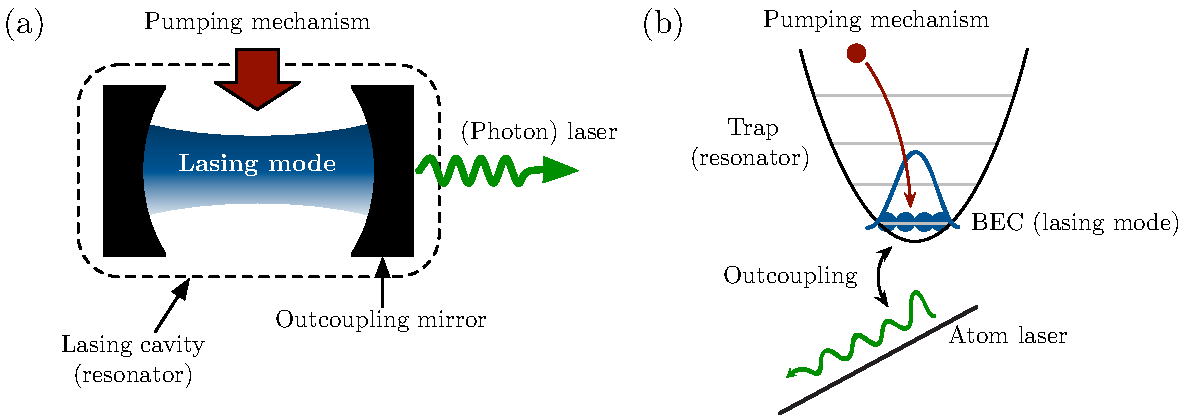
\includegraphics[width=14cm]{LaserAtomLaserComparison}
    \caption{
        \label{Introduction:LaserAtomLaserComparison}
        FIXME: This is not a caption.
    }
\end{figure}

\subsection{The resonator}
In an optical laser the resonator is typically an optical cavity formed between two (or more) mirrors trapping the photons within a region of space; the optical mode trapped within the resonator is the lasing mode.  For atom lasers the resonator is an `atom trap', either an optical trap using the ac Stark shift to trap the atoms in a region of high optical intensity, or a magnetic trap using the Zeeman shift to selectively trap certain magnetic hyperfine states near a local minimum of the magnetic field.

Discuss evaporation here?  Or maybe in the next section?

\subsection{The lasing mode}

The lasing mode of an atom laser is a BEC.  The lasing mode is of interest independently to the production of a continuous atom laser, as a Bose-Einstein condensate illustrates macroscopic quantum degeneracy of atoms.  Interesting quantum-mechanical effects that cannot be observed at higher temperatures... High degree of purity, controllability, stuff, nonsense.  I think I have stuff about this elsewhere.  All kinds of cool stuff you can do with a BEC.

\subsection{The outcoupling process}

Outcoupling light from the lasing mode in an optical laser is achieved through making one of the cavity mirrors partially transmittive, the emitted light is then the output mode of the optical laser. For atom lasers an analogous technique can be used for optical traps by lowering the depth of the trap until some atoms can tunnel out of the trap with the assistance of gravity. For atom lasers in magnetic traps a different technique is needed and either a microwave or Raman transition is employed to transfer the atoms into a magnetically-insensitive state that then falls under gravity. In addition to transferring the atoms into a magnetically-insensitive state, Raman transitions can also deliver a momentum kick to atoms that can be used to improve the spatial profile of the atom laser \cite{Jeppesen:2007yq}.

Here we discuss atom lasers in general.  We need to discuss spatial profile, and other things to do with (pulsed) atom lasers.

\subsection{Pumping mechanism}

Here we discuss pumping and matter-wave amplification.

Contemporary atom optics experiments operate in pulsed mode, and consistent with the analogy with a pulsed optical laser, these experiments are frequently limited by the linewidth (velocity-spread) of the atomic pulse produced. The present limit on this linewidth is proportional to the inverse of the outcoupling time for pulsed atom lasers \cite{Johnsson:2007}.  This limit can be made arbitrarily small (until the energy uncertainty in the BEC due to s-wave scattering becomes significant \cite{Johnsson:2007a}) at the expense of an arbitrarily small atom flux.  Practically, however, this trade-off cannot be made because the signal-to-noise ratio for these experiments depends critically on the atomic flux.  Alternatively, a continuous atom laser, in analogy to a continuous optical laser could operate for an arbitrary period of time independent of the atomic flux, hence reducing the linewidth of the atom laser until the s-wave scattering limit \cite{Johnsson:2007a} or a limit analogous to the Schawlow-Townes limit for optical lasers \cite{Schawlow:1958} was reached.


Without a pumping mechanism, an optical laser is simply a leaky cavity emitting an exponentially decaying amount of light with the same linewidth as the optical resonator.  The pumping mechanism for an optical laser not only permits the continuous operation of the laser, but it also narrows the linewidth of the laser below the bare cavity linewidth in a process known as \emph{gain-narrowing}. Gain-narrowing is caused by the saturation of the pumping process, and although a pumping process does not need to be saturable for the output of a laser to be coherent (or to have any other properties typically associated with a laser \cite{Wiseman:1997ba}), it is a useful property that would be convenient to have for atom lasers.


The other necessary property of a pumping mechanism is that the coupling process gives rise to a biased transfer of bosons from the pumping mode to the lasing mode.  In a generic laser pumping process (see \figureref{fig:PumpingMechanism}), one or two initial bosons are coupled with a Bose-enhanced coupling rate to a state with an additional boson in the lasing mode, and a secondary boson in a different state.  To prevent the possibility of this process removing bosons from the lasing mode, the state occupied by the secondary boson must be initially unpopulated, as if there were any population in this state it would be possible for the pumping process shown in \figureref{fig:PumpingMechanism} to run backwards.  Although this requirement will prevent any bosons being removed from the lasing mode, it does not guarantee that once a boson has been transferred to the lasing mode that it will not be removed again due to coupling back to the initial state.  To ensure that this does not occur, the secondary boson in the laser pumping process must irreversibly change state such that it can no longer interact in the pumping process, this is usually achieved by changing the internal state of the secondary boson or by removing it from the interaction region.  In an optical laser the initial boson is an atom in an excited state and it is coupled to a state where the atom has de-excited by emitting a photon into the lasing mode. To prevent the de-excited atom re-absorbing a lasing-mode photon and reversing the pumping process, this de-excited atom needs to rapidly change internal states. In a four-level laser pumping scheme this is achieved by ensuring that the atom in the de-excited state has a rapid, irreversible decay down to a lower state from which it can later be re-excited by the pump; in a three-level laser pumping scheme the de-excited atom is directly and irreversibly pumped to a highly-excited state.

\section{Pumping and Matter-wave amplification}

\section{Thesis overview}

\hrule

\section{Atom lasers}
\label{Introduction:AtomLaser}


\section{Pumping and (atom) lasers}
\label{Introduction:Pumping}

FIXME: This content to go in the introduction.

A brief overview of what gives a laser its properties. Refer to Wiseman's paper~\citep{Wiseman:1997ba} and compare the optical and atom lasers. Alternatives for the irreversibility / source are discussed in \chapterref{OpticalPumping,KineticTheory}.

There are two fundamental reasons making the pumping of an atom laser harder than pumping an optical laser is that the dispersion relation for potential reservoirs is not flat by comparison to the dispersion relation for atoms.  For an optical laser in the homogeneous broadening limit, \emph{all} atoms in the sample can contribute to gain.  Fundamentally this is because independent of what momentum the atom might have, it can still be stimulated to emit a photon into the lasing mode as the decay rates of the excited and/or ground atomic states are greater than any possible energy detuning in this process.  The second fundamental issue affecting atom lasers is that atom number is conserved.  It is therefore inescapable that there will be atoms in a (potentially) non-condensed source mode in the vicinity of the lasing mode.  Unless a Feschbach resonance is used to set the scattering-length of atomic interactions to zero, the atoms in the source mode will disrupt the phase stability of the lasing mode.

In \chapterref{OpticalPumping}, we attempt to solve the first problem by making the momentum distribution of source atoms sufficiently narrow that it can be guaranteed that every atom will be momentum-resonant with the pumping process at some point.  In \chapterref{KineticTheory}, we use atomic modes as the reservoir.  Although their dispersion relation cannot be flat with respect to that of the atoms in the source mode, it is at least far more comparable than that of light (which is used in \chapterref{OpticalPumping}).

Ideally we should pump an atom laser using something with a flat dispersion relation.  One possibility that comes to mind is the phonon.  However it is necessary that the reservoir is essentially a pure vacuum.  Phonons produced in a condensate cannot escape the system unless the system is in contact with other atoms.  If these other atoms are thermal, than it will have its own phonons which will propagate into the condensate.  If the condensate is not in physical contact with anything, then the phonons cannot leave the system: there is no evaporation process for phonons.

Stolen from \citep{Ballagh:2000oq}:
Despite the parallels with optical laser theory, the fundamental differences between photons and atoms remain important. They arise principally because atoms have rest mass, and because they interact with each other. Unlike photons, atoms cannot be created or destroyed, rather they are transferred into the laser mode from some other mode. The interactions produce phase dynamics, which degrades the coherence of the atom laser, and self repulsion which spreads the output beam and limits the possible focussing. Even when these interactions are neglected, atoms have dispersive propagation in vacuum.
